\documentclass[12pt, a4paper]{article}
\usepackage[T1]{fontenc}
\usepackage[utf8]{inputenc}
\usepackage{graphicx, textcomp, gensymb, tabularx, booktabs, wrapfig, indentfirst, amsmath, geometry, amssymb, caption}
\usepackage[backend = biber]{biblatex}
\newgeometry{tmargin=2cm, bmargin=2cm, lmargin=2cm, rmargin=2cm}
\renewcommand{\figurename}{fig.}


\begin{document}

\title{
	\textbf{Model konceptualny projektu \\ 
	Bazy danych 2019} \\
	Prowadzący: dr Małgorzata Biernacka}
	
\author{
	Maciej Draguła \\
}

\date{30 maja 2019}


\maketitle

\section{Diagram E-R}

\begin{figure}[h!]
	\centering
	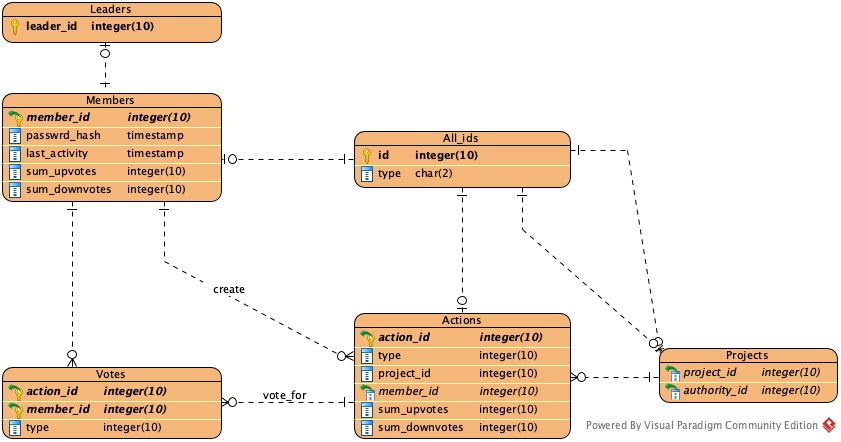
\includegraphics[width = 17cm]{diagram.jpg}
	\caption{}
\end{figure}

\section{Komentarz}

W projekcie wyróżniamy dwa rodzaje logowania do bazy danych - logowanie jako tzw. \textit{member} albo jako \textit{leader}. Leader ma wgląd w całą bazę danych, tzn. może odpytywać o jej elementy, agregować i prezentować wyniki, ale również ma uprawnienia membera. Member może natomiast tylko oddawać głosy i wdrażać nowe akcje. Uwierzytelnianie użytkowników będzie się obywało poprzez sprawdzenie zgodności hasha podanego hasła i (potencjalnie) odpowiadającemu mu w bazie danych.

Każdy użytkownik może oddać głos, czyli stworzyć nowy element w tabeli \textit{Votes}, co uruchomi wyzwalacz, który uaktualni wartości \textit{sum upvotes} albo \textit{sum downvotes} w tabeli \textit{Actions}. Zmiana jednej z tych dwóch wartości będzie uruchamiać kolejny wyzwalacz, który uaktualni wartości \textit{sum upvotes} albo \textit{sum downvotes} w tabeli \textit{Members}.

Poszczególne funkcje API będą wywołaniami SQL odpowiednio uzupełniającymi tabele bądź odpytującymi o zadane wartości.

Aby sprawdzić, czy użytkownik jest aktywny należy upewnić się, czy czas, który upłynął od timestampu aktualnie dodawanej akcji bądź oddawanego głosu, jest dłuższy niż rok (tzn. czy jest oddalony o więcej niż rok od pola \textit{last activity} w tabeli \textit{Members}).

Typem głosowań jest \textit{support}(1) albo \textit{protest}(-1), natomiast typem id jest \textit{member}(mb), \textit{leader}(ld), \textit{action}(ac), \textit{project}(pj) lub \textit{authority}(au). Ponadto zostanie zadbane również o to, aby każdy użytkownik na konkretną akcję mógł oddać co najwyżej jeden głos.

\end{document}